\chapter{Design}
	The most important aspects of the selected solution are documented in this chapter.

	\section{Software Architecture}
		As there weren't any special architectural requirements needed for RaceTrack, it was decided to opt for a \textbf{layered architecture}. For the development of RaceTrack, the UI will be separated from the model and application logic. This layered architecture will be used to separate the application's concerns into two stages:
		\begin{itemize}
			\item \textbf{User Interface} represents the visualization of the data that model contains \textit{(package com.pathfinder.racetrack.view)}.
			\item \textbf{Domain- / Application Logic} acts on both model and view. It controls the data flow into model objects and updates the view whenever data changes. It keeps view and model separate \textit{(package com.pathfinder.racetrack.model)}.
		\end{itemize}
		\begin{figure}[H]
			\centering
			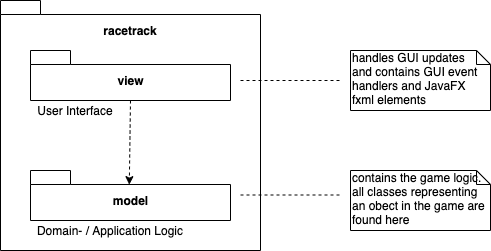
\includegraphics[width=12cm,keepaspectratio,center]{img/Software-Architecture_MVC-Custom.png}
			\caption{Layered implementation in RaceTrack}
		\end{figure}
		Not only does this abstraction separate the different aspects of the application, but it also provides loose coupling between these elements. The UI logic belongs in the view and business logic belongs in the model. Because of the separation of responsibilities, future development or modification is also easier. This layered architecture will also be easier to implement in a game, as other patterns like a pure implementation of the MVC Pattern are really difficult to implement using Java and especially JavaFX. \\~\\
		
		\newpage
		
		\textbf{Package Diagram:} \\
			\begin{figure}[H]
				\centering
				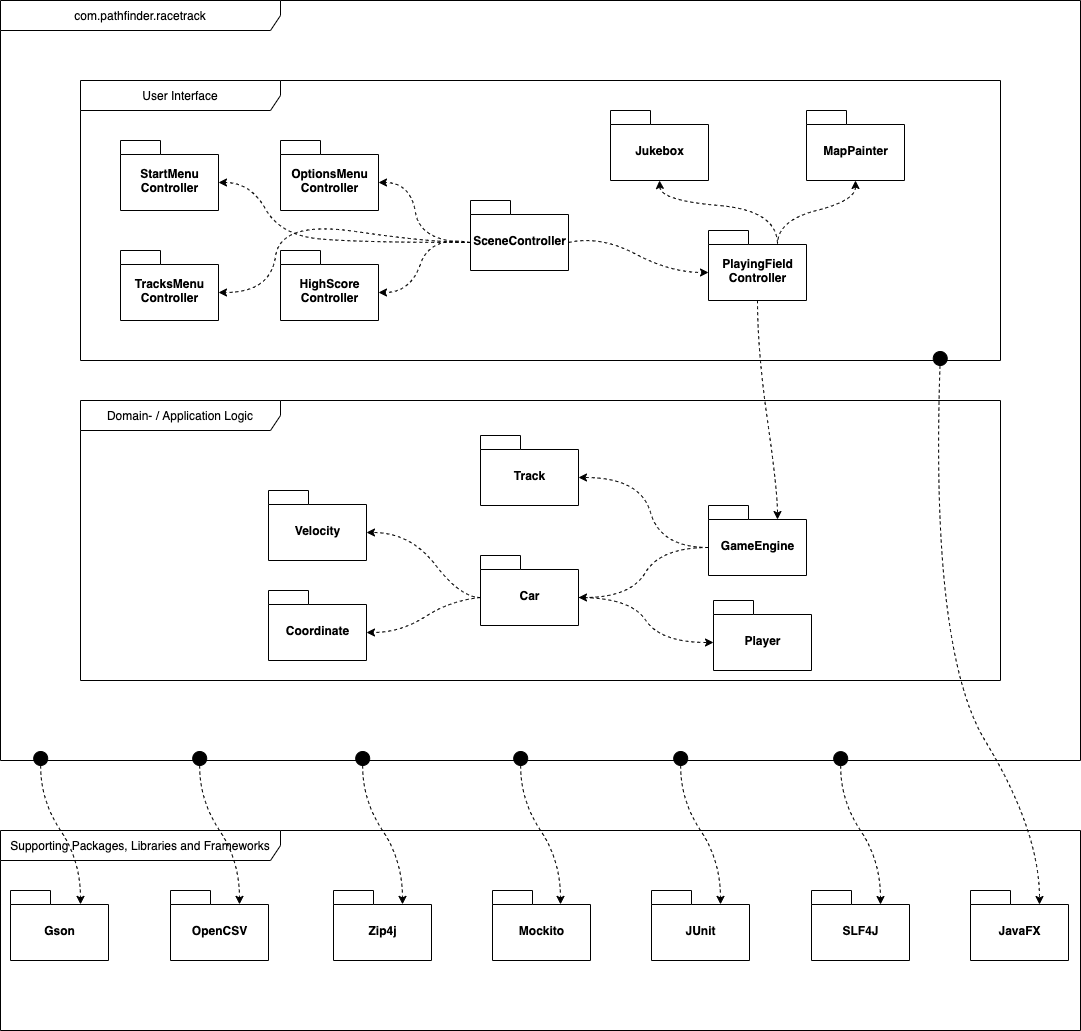
\includegraphics[width=16cm,keepaspectratio,center]{img/Software-Architecture_UML-Package-Diagram.png}
				\caption{Package Diagram of RaceTrack}
			\end{figure}

		\subsection{Distribution Model}
		As RaceTrack will be played on a single device, there isn't any need for a distribution model. But the game will be implemented to allow distributed sessions (Peer-to-Peer) in the future.